\chapter{Introduction}
\section{Preamble}
This literature review provides background for the data mining toolkit I am developing to extend the open-source framework for automated collection of the software development process data named Hackystat. Hackystat gathers data about human activity (developers' behavior) and various code metrics indicating size, structure and quality of the code. After transformation and aggregation of the raw sensor data Hackystat stores it in a temporal database providing users with infrastructure for the retrieval and visualization of the telemetry data. It is possible not only to select a desired data granularity but also to refine telemetry streams by specifying individual or groups of developers, set of projects as well as individual metrics and their derivatives. While all of this provides a rich environment for the analysis and interpretation of the software development process, the comparison of telemetry streams is still performed by ``eyeballing'' and thus automation is a highly desirable feature. Once processing of range queries is implemented, it will allow extension of the analysis toolkit with various KDD methods aiming but not limited to indexing, clustering\footnote{We are aware of controversal views on the clustering of time-series expressed in \cite{citeulike:227029} by Keogh et al.}, software development pattern discovery and real time sensor data stream analysis.

\section{Introduction to time-series}
The time-series is a data type represented by a sequence of data points sampled at successive times and usually found as the sequence of real or integer numbers with or without attached timestamps. Time-series data arises naturally from observations and reflects an evolution of some subject or a development of some phenomena in time. Since the time-series is the only way to store valuable and often non-reproducible temporal information, it makes time-series data ubiquitous and important not only in every scientific field but also in everyday life. For example, it is very common to see visualized time-series representing financial information about stocks and currency fluctuations, weather changes or social trends in newspapers or TV programs. Medical observations, such as blood pressure, heart beat rate or a body temperature changes is another example of time-series commonly seen in life. According to Tufte \cite{citeulike:1454223} ``The time-series plot is the most frequently used form of graphic design. With one dimension marching along to the regular rhythm of seconds, minutes, hours, days, weeks, months, years, or millennia, the natural ordering of the time scale gives this design a strength and efficiency of interpretation found in no other graphic arrangement.'' The figure \ref{fig:10century} from the Tufte book depicts the oldest known example of a time-series plot showing the planetary orbits inclinations and is dated back to the tenth century.
\begin{figure}[tbp]
   \centering
   \includegraphics[height=70mm]{10century.eps}
   %%{seriesheatmap}
   \caption{Ancient time-series plot showing the planetary orbits inclinations.}
   \label{fig:10century}
\end{figure} 

It is generally assumed that consecutive measured values in a time-series are sampled at equally spaced time intervals (which is not always true and if required, resampling and interpolation can be used). This specific ordering of sample values in time often provides valuable information about the dependency of successive observations on earlier ones and is the key feature distinguishing time-series data from usually independent statistical samples. 
The explicit recognition of ordering in time-series analysis techniques makes them somewhat different from traditional statistical analyses \cite{citeulike:3989988}. It should be noted - that while many time-series analysis methods treat time-series as simple sequences of real numbers discarding the actual time-stamps, the time-ordering is always considered and it is assumed that unpronounced time interval are equal between the sampled values.

Time-series analysis methods in general combine various statistical and pattern recognition techniques while using information presented in the time-ordering of samples. Historically, time-series analysis is divided by two major fields of study: the first is explorative and descriptive analysis and the second is forecasting. 
While the descriptive analyses focus on the understanding of the time-series generating processes itself by finding trends, periodicity and some hidden features within the time-series \cite{citeulike:2206845}, the predictive analyses aim at forecasting the future of the time-series generating process based on the information found by conducting descriptive analyses \cite{citeulike:3449765}. 
Both - descriptive and predictive analyses are based on the identification of some pattern in the time-series which can be formally described and can correspond to the time-series generating process. Once this pattern is found and compiled into the formal model during the explorative analysis, it is used for extrapolation of the time-series into the future. Such  model development and forecasting can be traced from the Babylonian astrologist predicting celestial phenomenas to the contemporary stochastic and deterministic models in many scientific fields.

As we mentioned before, time-series are ubiquitous. Taking into account the fact that most of the data collected automatically by sensing and monitoring are time series, it is hard not to overemphasize the importance and value of time-series data and analyses. Many public and private time-series databases exist for tracking and analysis of various information, and contemporary trends in the cost of data storage, increased bandwidth and progress in information science enable tremendous growth in time-series data volume and variety. There are public databases which track financial indexes and climate change (Figure \ref{fig:onlineDB}), astronomical observations \cite{citeulike:4373331}, medical information \cite{citeulike:4373332} and many others.  This growth in temporal data volume and availability during the last decade of the twentieth century have created a demand for new approaches in KDD (Knowledge Discovery and Data mining) applications capable of handling very large volumes of temporal data. Since most KDD techniques such as classification, clustering and pattern discovery are based on the ability to quantify similarity between subjects, the need for advanced algorithms created a whole new research field dealing with data mining in temporal databases. Much research work has been done in the past 20 years, resulting in more than a dozen core algorithms which can be further extended for specific needs. In this work we will review the most relevant ones in order to understand their ability to perform in our application domain.

\begin{figure}[tbp]
   \centering
   \includegraphics[height=190mm]{onlineDB.eps}
   %%{seriesheatmap}
   \caption{Examples of time-series databases. Upper screenshot is the FRED (Federal Reserve Economic Data) database of 20,056 U.S. economic time series, lower is the part of the NOAA Climate time-series database.}
   \label{fig:onlineDB}
\end{figure} 
